% Picar el capitulo entre Implementacion y Experimentos
% Añadir un p\'arrafo al final de Implementacion de como se utilza el nuevo sistema
\chapter{AutoGOAL Multiobjetivo}\label{chapter:implementation}
AutoGOAL (\cite{estevez2020solving}) es un sistema AutoML Heter\'ogeneo modular y f\'acilemente extensible. Modela su espacio de b\'usqueda utilzando Gram\'aticas Probabil\'istica  Libre del Contexto (PCFG, \cite{megane2021probabilistic}), una extensi\'on de las Gram\'aticas Libres del Contexto al asignar a cada producci\'on una probabilidad. Con el fin de dirigir la b\'usqueda utiliza \textit{Probabilistic Grammatic Evolution} (PGE), una modificaci\'on de \textit{Grammatical Evolution}
%basada en Algoritmos de Estimaci\'on de Distribuci\'on (EDAs)
para ser usada con PCFG.

PGE est\'a basado en Algoritmos de Estimaci\'on de Distribuci\'on (EDAs) una t\'ecnica evolutiva que remplaza las operaciones de mutaci\'on y cruce por un muestrado sobre las probabilidaes de las producciones de PCFG. Dado una gram\'atica $G$ y una cadena $c \in G$, PGE modifica las probabilidades asociadas a cada producci\'on de $G$ para que las proximas generaciones que utilizen $G$ tengan mayor probabilidad de utilizar las mismas producciones que $c$. Cuando $c$ representa el individuo m\'as aptos entonces las pr\'oximas generaciones tienen mayor probabilidad de conservar sus caracter\'isticas.
Este es un algoritmo sencillo pero efectivo que logra un balance entre exploraci\'on y explotaci\'on local haci\'endolo resistente a m\'inimos locales y a la generaci\'on de soluciones iguales.

\section{Implementaci\'on}

\begin{figure}[ht]
    \centering
    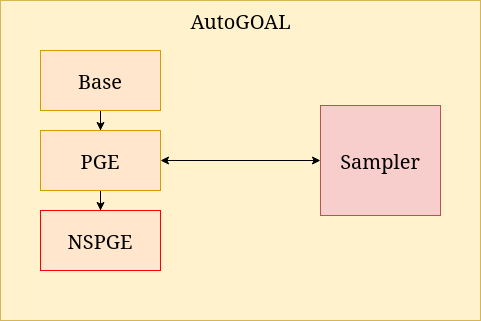
\includegraphics[scale=0.6]{Pictures/autogoal_impl.png}
    \caption{Diagrama general}
    \label{impl:fig:general_diagram}
\end{figure}


La manera de AutoGOAL de representar su PCFG utilizada para modelar su espacio de decisi\'on es utilizando un grafo aciclico dirigido (DAG) donde cada nodo representa una posible cadena de la gram\'atica y sus aristas apuntan a todas las posibles cadenas a las que se puede expandir sustituyendo alg\'un No Terminal por una producci\'on de la Gram\'atica correspondiente. Cuando una cadena se encuentra completamente expandida, i.e. compuesta por solo simbolos terminales, se tiene una soluci\'on v\'alida del sistema. 

Inicialmente cada arista del DAG se inicializa con una probabilidad igual a todas sus aristas hermanas (i.e. todas las aristas que salen de su mismo nodo) tal que la suma de sus probabilidades sea 1. Un camino se escoge utilizando una variable uniforme donde su valor determina la arista a seleccionar.
Una vez que se tiene un individuo apto AutoGOAL aplica PGE sobre el grafo actualizando las probabilidades de todas las aristas seg\'un el camino utilizado por dicho individuo. Esta operaci\'on se realiza sobre los $k$ individuos m\'as aptos de la poblaci\'on generada. %PGE en AutoGOAL utiliza una lista de los $k$ individuos m\'as aptos para actualizar el grafo.
% Cuando se tiene un individuo apto la manera de AutoGOAL de conservar sus ``genes'' es aplicando PGE sobre las aristas que conforman el camino que condujo a esa soluci\'on. M\'as especificamente, la implementaci\'on de AutoGOAL de PGE dado $n$ individuos, son evaluados respecto a un criterio de evaluaci\'on $f$ y se crea una lista de las $k$ mejores soluciones (encabezada por la m\'as apta) y las aristas de las probabilidades se actualizan de acuerdo a estas soluciones. 

\subsection{NSPGE}
NSPGE, un algoritmo de b\'usqueda inspirado en NSGA-II (\cite{deb2002fast}), define una nueva ordenaci\'on sobre las soluciones generadas por AutoGOAL. Se define como una clase que hereda directamente de PGE con el objetivo de extender la l\'ogica de PGE encargada de seleccionar los $k$ mejores individuos de acuerdo a $m$ m\'etricas, con $m \ge 2$. PGE define su simple l\'ogica de seleccion dentro del m\'etodo \textit{\_inidices\_of\_the\_fittest\_} el cual NSPGE sobreescribe.

La redefinici\'on \textit{\_inidices\_of\_the\_fittest\_} incluye las dos etapas de ordenaci\'on definida por \cite{deb2002fast}. Dado $n$ soluciones se  agrupan seg\'un su \'indice de dominaci\'on (i.e. Non Dominated Sorting), donde cada agrupamiento se le llama frente de rango $i$, donde $i$ representa la cantidad de soluciones que dominan a cada una de estas. Una vez establecidos estos frentes se extraen las primeras $k$ soluciones, en caso de que no se pueda seleccionar un frente completo, se aplica Crowding Distance para seleccionar la muestra m\'as representativa de este.


\begin{lstlisting}[caption=Nueva ordenaci\'on, language=Python]
def _indices_of_fittest(self, fns: List[List[float]]):
  # Se ordenan todas las soluciones segun su orden
  # de dominacion
  fronts = self.non_dominated_sort(fns)
  indices = []
  k = int(self._selection * len(fns))

  for front in fronts:
    if len(indices) + len(front) <= k:
      indices.extend(front)
    else:
      # Cuando solo se utiliza una porcion del frente
      # se aplica crowding distance
      indices.extend(
          sorted(
              front,
              key=lambda i: -self.crowding_distance(fns, front, i)
          )[: k - len(indices)]
      )
      break
  return indices
\end{lstlisting}

\subsubsection{Non Dominated Sort}
La ordenaci\'on se conforma por dos pasos l\'ogicos fundamentales:
\begin{enumerate}
    \item Se verifica todo par de soluciones $x, y$ encontradas y se aplica $x \prec y$ con el objetivo de calcular el \'inidice de dominaci\'on de cada soluci\'on. Adem\'as se construye un DAG conformado por las soluciones donde existe una arista entre las soluciones $x$ y $y$ si $x \prec y$. La ra\'iz de dicho DAG est\'a conformado por las soluciones que nadie domina.
    \item Se recorre DAG utilizando una versi\'on de BFS (\textit{Breadth First Search}) partiendo por las soluciones que tienen \'indice de dominaci\'on 0. Todas las soluciones visitadas se le es reducido el \'indice de domianci\'on en uno. Si llega a 0 se a\~nade al frente de Pareto que se est\'a formando. Luego se comienza el proceso nuevamente partiendo por las soluciones a las cuales su \'indice se redujo a 0.
\end{enumerate}

\begin{lstlisting}[caption=Non Dominated Sorting, language=Python]
def non_dominated_sort(self, scores: List[List[float]]):
  # fronts almacena los frentes 
  #(i.e. fronts[i] es el frente de rango i)
  fronts: List[List[int]] = [[]]

  # domination_rank en i indica la cantidad de soluciones
  # que dominan a la solucion i
  domination_rank = [0] * len(scores)

  # dominated_scores en i alamacena las soluciones dominadas
  # por la solucion i
  dominated_scores = [list() for _ in scores]

  # revisa todo par de soluciones y se establece
  # quien dominan a quien
  for i, score_i in enumerate(scores):
    for j, score_j in enumerate(scores):
      if self._improves(score_i, score_j):
          dominated_scores[i].append(j)
      elif self._improves(score_j, score_i):
          domination_rank[i] += 1
    if domination_rank[i] == 0:
       fronts[0].append(i)

  # de acuerdo a la informacion sobre quienes
  # se dominan, forma todos los frentes
  front_rank = 0
  while len(fronts[front_rank]) > 0:
    next_front = []
    for i in fronts[front_rank]:
      for dominated in dominated_scores[i]:
        domination_rank[dominated] -= 1
        if domination_rank[dominated] == 0:
          next_front.append(dominated)
    front_rank += 1
    fronts.append(next_front)

  return fronts[:-1]
\end{lstlisting}

\subsubsection{Crowding Distance}
Se sigue la idea del algoritmo propuesto en (\ref{proposal:alg:cd}). Dado $m$ m\'etricas a evaluar se realizan $m$ iteraciones, donde en cada una se ordena un frente de rango $k$ de acuerdo a la metrica $m_i$. Las soluciones que con respecto a la m\'etrica $m_i$ tienen el m\'inimo y mayor valor se les asigna distancia infinita y luego se c\'alculan los valores intermedios. En \cite{deb2002fast} requiren que las componentes de los vectores soluci\'on esten normalizadas antes de ejecutar \textit{Crowding Distance}, en nuestra implementaci\'on utilizamos \textit{feature scaling} para normalizar los valores entre 0 y 1.

\begin{lstlisting}[caption=Crowding Distance Sorting, language=Python]
def crowding_distance(
    self, scores: List[List[float]], front: List[int], index: int
) -> float:
  # Crowding distance usa los vectores normalizados.
  # Se aplica feature scaling para llevar cada
  # componente de los vectores al rango [0, 1]
  scaled_scores = feature_scaling(scores)

  crowding_distances: List[float] = [0 for _ in scores]
  for m in range(len(self._maximize)):
    # Se ordena de acuerdo a la metrica m
    front = sorted(front, key=lambda x: scores[x][m])

    # Se establecen los extremos como infinitos
    crowding_distances[front[0]] = math.inf
    crowding_distances[front[-1]] = math.inf

    # Valores de todas las soluciones con respecto a m 
    m_values = [scaled_scores[i][m] for i in front]
    scale: float = max(m_values) - min(m_values)
    if scale == 0:
      scale = 1
    for i in range(1, len(front) - 1):
      crowding_distances[i] += (
        scaled_scores[front[i + 1]][m] - scaled_scores[front[i - 1]][m]
      ) / scale

  return crowding_distances[index]
\end{lstlisting}

\section{Aplicaci\'on de Autogoal Multiobjetivo}
AutoGOAL Multiobjetivo mantiene la misma interfaz que AutoGOAL. Para utilizar esta nueva ordenaci\'on se necesita  se\~nalar el algoritmo de b\'usqueda a utilizar con el par\'ametro \textbf{search\_algorithm}.Adem\'as es necesario definir una m\'etrica que retorne 2 o m\'as valores en \textbf{score\_metric} y especificar por cada una si se desea maximizar o minimizar utilizando el par\'ametro  \textbf{maximize}. 

\begin{lstlisting}[caption=Utilizando NPSGE, language=Python]
from autogoal.datasets import cars
from autogoal.kb import (
  MatrixContinuousDense,
  Supervised,
  VectorCategorical
)
from autogoal.ml import AutoML
from autogoal.search import NSPESearch

automl = AutoML(
    input=(MatrixContinuousDense, Supervised[VectorCategorical]),
    output=VectorCategorical,
    search_algorithm=NSPESearch, # Algoritmo de Busqueda
    score_metric=accuracy_vs_time, # Metrica de varios criterios
    maximize=(True, True), # Componentes de la metrica a maximizar
)

# Entrena el modelo
x, y = cars.load()
automl.fit(x, y)

# Imprime todas las soluciones encontradas
print(automl.best_pipeline_) 
\end{lstlisting}

\subsection{M\'etricas}
La definici\'on de las m\'etricas es similar a como se definen en AutoGOAL est\'andar con la diferencia de que estas retornan tuplas de elementos.

\begin{lstlisting}[caption=Ejemplo de m\'etrica: accuracy contra tiempo, language=Python]
from time import time
import autogoal.ml.metrics as metrics

def acc_vs_train_time(*args, **kwargs):
    t1 = time()
    acc = metrics.accuracy(*args, **kwargs)
    t2 = time()
    score = [acc, t1 - t2]
    return score
\end{lstlisting}
